\subsection{Automated testing}

This section is mainly useful for the develpers or those want to change/add/remove some parts of the code and compare the new changes with the reference solutions.
For the reference solutions, 5 different tests have been designed and 
the results from \textit{yspec} [Al-Attar \& Woodhouse (2008)] and AXISEM have been included in the \textit{TESTING/automatic} directory.
The whole procedure (running the code, compare the results and plot) is automatic with the least user intervention: \\

Start from within the {\tt AXISEM} directory:
 \begin{enumerate}
 \item {\tt cd TESTING}
 \item {\tt python test\_axisem.py}
 \end{enumerate}

Enter test number(s) and this is all you should do! \\

\noindent As an example, we want to run the script \textit{test\_axisem.py} for test number 5. (Figure~\ref{test_axisem})

\begin{figure*}[htb]
  \begin{verbatim}
   ==========================================
  Please enter the test number(s): 
  1. test01: explosion
  2. test02: dipole (mxz)
  3. test03: quadpole (mxy)
  4. test04: CMT (location: north pole)
  5. test05: CMT (location: 70°N 50°E)

  (format = 01,02 OR 1,2,3)
  \end{verbatim}
  \caption{\textit{Screenshot while running test\_axisem.py}}
\label{test_axisem}
\end{figure*}

\noindent At the end, it plots three figures (one for each channel) 
in which the new AXISEM waveforms are compared with both the original ones and \textit{yspec} results for the same simulation.
%In Figure~\ref{channel_Z}, only the Z channel has been plotted.
It should be noted that these tests are designed for rough comparison purposes (in terms of the pulse shape and sign) and they should not be considered as a detailed benchmark with respect to YSPEC. \\

\begin{figure}
  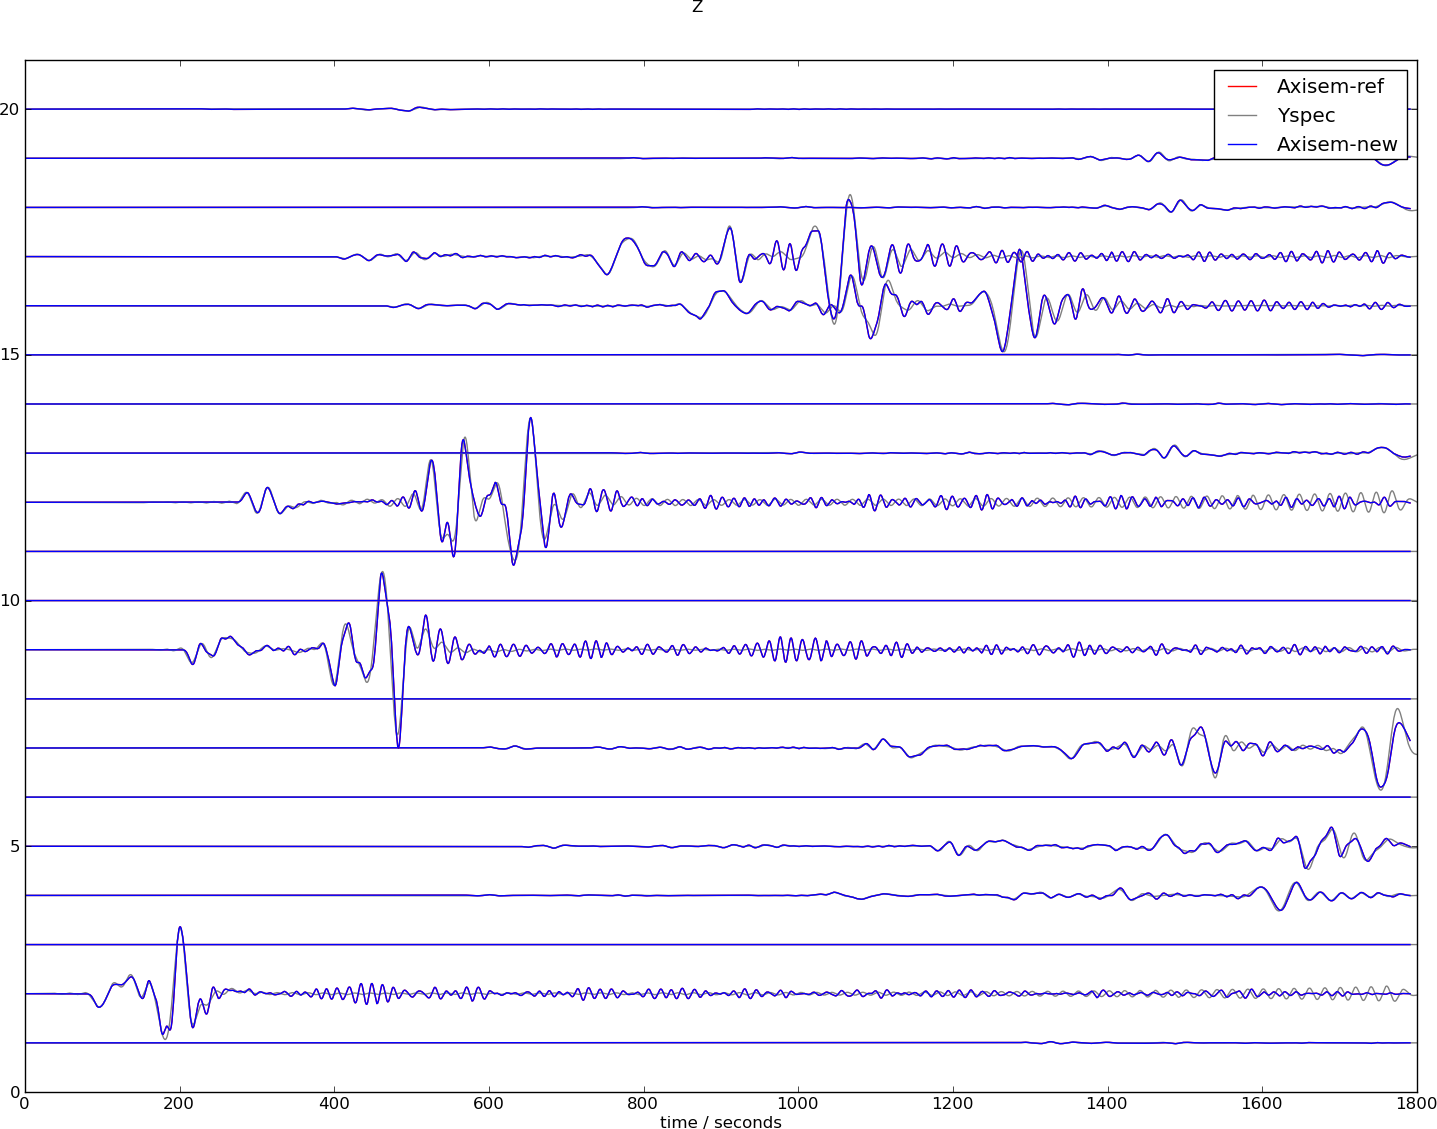
\includegraphics[width=0.48\textwidth]{./PYAXI/record_section_Z.png}
  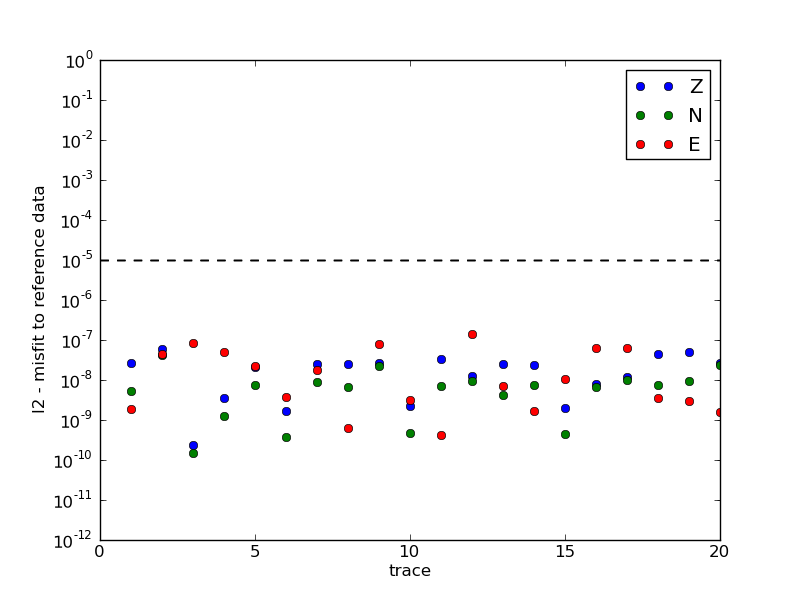
\includegraphics[width=0.48\textwidth]{./PYAXI/l2_misfit.png}
  \caption{\textit{Comparing new AXISEM results with the reference solution and \textit{yspec} waveforms. (Z channel)}}
  \label{channel_Z}
\end{figure}

\noindent Another output is the RMS misfit (Figure~\ref{l2_misfit}) between the new and reference data 
in which the traces can be compared in a quantitative sense.

% \begin{figure}
% 
%   \caption{\textit{RMS misfit between the new and reference data.}}
%   \label{l2_misfit}
% \end{figure}
